\documentclass[10pt]{article}
\usepackage{amsmath}
\usepackage[margin=3cm]{geometry}
\usepackage[colorlinks=true, linkcolor=blue]{hyperref} 
\usepackage{listings}
\usepackage{color}
\usepackage[style=authoryear, citestyle=authoryear]{biblatex}
\usepackage{graphicx}
\usepackage[labelfont=bf]{caption}

\definecolor{gray}{rgb}{0.95,0.95,0.95}
\lstset{
    tabsize=4,
    backgroundcolor=\color{gray},
    upquote=Truet,
    basicstyle=\small
}

\title{Technical report on the test particle simulations}
\author{Mathew Bub}
\date{\today}

\addbibresource{ref.bib}

\begin{document}
\maketitle

This report provides a technical overview and summary of our work on high resolution test particle simulations of non-axisymmetric Galactic structures, including the Galactic bar and spiral arms. In Section \ref{tech}, we provide a technical overview of the test particle simulations, including the tools utilized to integrate the test particles, as well as the setup of the initial conditions. In Section \ref{scinet}, we discuss the additional tools utilized to run these simulations on the SciNet Niagara supercomputer. Finally, in Section \ref{results}, we consider the results of a select number of simulations.

\section{Technical overview} \label{tech}

\subsection{Orbit integration} \label{integration}
All large orbit integration suites were computed using \texttt{galpy}'s \texttt{Orbits} class, a recent addition which allows for many orbits to be integrated in parallel. As of this writing, \texttt{Orbits} is available \href{https://github.com/jobovy/galpy/tree/orbits}{here} in the \texttt{orbits} branch of \texttt{galpy}. In the future, it is expected that \texttt{Orbits} will be combined seamlessly with the existing \texttt{Orbit} class.

In addition to \texttt{Orbits}, we developed additional tools to integrate very large numbers of orbits in a series of chunks, in order to handle the large memory requirements of such computations. These tools have been included in a small Python package called \texttt{multiorbit}, which is available on \href{https://github.com/mwbub/multiorbit}{github}. The main tool available in this package is the \texttt{integrate\_chunks} function, which accepts as input the initialization parameters for an \texttt{Orbits} object, as well as a potential and a time array, and integrates the initial conditions in parallel. The function also periodically saves the results of the integration to a \texttt{.fits} file, allowing the integration to be resumed in case of interruption. Full documentation for this function is available on github.

\subsection{Setup of the initial conditions} \label{init}
The initial conditions for the test particle models were sampled using \texttt{galpy}'s \texttt{quasiisothermaldf}, a distribution function adapted from \textcite{B10} which is expressed in terms of action-angle variables. The specific setup of the distribution function was as follows:
\begin{lstlisting}[language=Python, numbers=left]
from galpy.df import quasiisothermaldf
from galpy.potential import MWPotential2014
from galpy.actionAngle import actionAngleStaeckel

# Set up QDF object
aA = actionAngleStaeckel(pot=MWPotential2014, c=True, delta=0.45)
qdf = quasiisothermaldf(1./3., 0.15, 0.075, 1., 1., pot=MWPotential2014, 
                        aA=aA, cutcounter=True)
\end{lstlisting}
This code snippet sets up a QDF object with a radial scale length of $R_0/3$, a local radial and vertical velocity dispersion of $0.15 \times V_\mathrm{c}(R_0)$ and $0.075 \times V_\mathrm{c}(R_0)$, respectively, and a radial scale length of $R_0$ for the velocity dispersions. In addition, counter-rotating stars are explicitly excluded from the distribution function. Action-angles are calculated using the Staeckel approximation via \texttt{galpy}'s \texttt{actionAngleStaeckel}, and the potential is evaluated with \texttt{MWPotential2014}.

Using this distribution function, we generated $2 \times 10^8$ position and velocity samples between Galactocentric radii of 1 and 13 kpc. Positions were sampled by computing \texttt{qdf.density} over a grid of points in space containing the sampling region, interpolating these points to generate a continuous approximation of the DF, and then performing the random sampling. Velocities were sampled using the built-in \texttt{qdf.sampleV\_interpolate} method, which performs a similar procedure for the velocities. The sampled initial conditions were saved in a \texttt{.fits} files containing columns labelled \texttt{R}, \texttt{phi}, \texttt{z}, \texttt{vR}, \texttt{vT}, and \texttt{vz}, representing the Galactocentric cylindrical coordinates of each test particle.

When the initial conditions were sampled, it was noted that the resultant disk of test particles was significantly out of equilibrium when integrated with \texttt{MWPotential2014}, despite having been sampled while assuming that same potential. To correct this, we integrated the test particles forward in time for 7 Gyr in \texttt{MWPotential2014} prior to integrating any other models, to allow the disk to reach equilibrium. This relaxation period had a side effect of shifting the mean azimuthal velocity at the Solar radius from approximately 220 km s$^{-1}$ to approximately 200 km s$^{-1}$.
 
\section{SciNet integration} \label{scinet}
In addition to the computational tools described in Section \ref{tech}, a number of additional tools were used to perform the orbit integration on the SciNet Niagara cluster specifically. General instructions about setting up \texttt{galpy} on SciNet can be found \href{https://github.com/mwbub/scinet-setup}{here}. When specifically running large orbit integration suites on SciNet, it is important to consider the behaviour of the Niagara job priority queue. In general, when submitting jobs to SciNet without a group resource allocation, it is most efficient to split a single large job into a number of small jobs that run for a short time on a small number of nodes. Thankfully, when integrating test particles in a fixed potential, the integration suites can be divided into arbitrarily small batches which run on separate nodes. Therefore, we perform our integration suites by submitting several hundred single-node jobs which each run for less than 4 hours. 

To streamline this process, we also include a function called \texttt{integrate\_batch} in the \texttt{multiorbit} package for automatically dividing a test particle integration suite into many small batches. The function accepts as parameters a time step array, a potential, and the name of an initial conditions \texttt{.fits} file, and automatically integrates a single batch of the initial conditions by calling \texttt{integrate\_chunks}. It also accepts keyword arguments to indicate the chunk size to pass to the \texttt{integrate\_chunks}, and a Boolean flag indicating whether to save all time steps, or only the final time step.

When running a Python script which calls \texttt{integrate\_batch}, you must provide three command line arguments to the script. The first argument is an integer which tells the function which batch it should integrate. The second argument represents the total number of batches into which the initial conditions are to be divided. The final argument is the name of the directory to which the function will save the results of the integration. A typical command line call to a script \texttt{integrate.py} which calls \texttt{integrate\_batch} would therefore look like this:
\begin{lstlisting}[language=bash]
$ python integrate.py 50 200 $SCRATCH/data/results
\end{lstlisting}
This line indicates to \texttt{integrate\_batch} that it should divide the initial conditions into 200 batches, and that this particular call to the script should integrate the 50$^{\mathrm{th}}$ batch. The function would then create a folder titled \texttt{batch50} in the \texttt{\$SCRATCH/data/results} directory, which would contain the output of \texttt{integrate\_chunks} when applied to the indicated batch of test particles. An example of a typical file which makes a call to \texttt{integrate\_batch} would be as follows:
\begin{lstlisting}[language=Python, numbers=left]
import numpy as np
from multiorbit import integrate_batch
from galpy.potential import # some potentials

# set up your potential here
t = np.linspace(start, end, num_timesteps)
integrate_batch(t, pot, initial_conditions_file, save_all=True)
\end{lstlisting}

The reason why we use command line arguments to divide the initial conditions is to take advantage of the array job feature in the SLURM workload manager, which is what Niagara uses to schedule jobs. When submitting a job script to SLURM using the \texttt{sbatch} command, you can also include the \texttt{-a <indices>} flag to indicate that the desired job is an array job. Array jobs are used when many similar jobs must be submitted with slightly different parameters. In our case, we wish to submit many jobs to integrate a set of initial conditions, each job integrating a different batch. The various jobs in a job array can be distinguished with the \texttt{\$SLURM\_ARRAY\_TASK\_ID} variable, which corresponds to the array indices passed to \texttt{sbatch}. Here, we use the array indices to indicate which batch each job in an array job should integrate. Thus, an example of a typical job submission script \texttt{job.sh} would be:
\begin{lstlisting}[language=bash, numbers=left]
#!/bin/bash
#SBATCH --nodes=1
#SBATCH --ntasks=80
#SBATCH --time=03:00:00
#SBATCH --job-name integrate-orbits
#SBATCH --mail-user=your.email@mail.utoronto.ca
#SBATCH --mail-type=ALL

module restore myModule
source activate myVirtualEnv

cd /path/to/directory/with/python/script/

python integrate.py $SLURM_ARRAY_TASK_ID 200 $SCRATCH/data/results
\end{lstlisting}
When we submit this job, we would run the following command in the command line:
\begin{lstlisting}[language=bash]
$ sbatch -a 1-200 job.sh
\end{lstlisting}
This line submits 200 separate jobs to the SLURM queue, each of which integrates a single batch of the initial conditions out of 200 total batches. A detailed description of each line in the \texttt{job.sh} script is as follows:

Lines 2 and 3 of the script indicate that we are submitting a job which uses a single node to run 80 threads. Note that although each node has 40 CPU cores, we can run up to 80 threads by using ``hyperthreading'', which can improve computational efficiency in certain circumstances. 

Line 4 indicates that each job submission is given a maximum wall time of 3 hours. The time required to run a single batch of an integration suite depends on the potential being used and the number of particles being integrated in each batch. To estimate this number, the general wisdom is to observe how long a previous batch takes to run, and add about 20\% to this number as a safety buffer. Try to minimize the maximum wall time assigned to each job, as this affects the priority of the job in the SLURM queue.

Lines 5-7 indicate the name of the job as well as an email address to which updates about the status of the array job will be sent. When using an array job, an email will be sent only when the first job in the array begins and when the last job finishes, as opposed to sending a separate email for every single job.

Lines 9 and 10 load a series of software modules required to run \texttt{galpy}, and activate the associated Python virtual environment. An explanation of the Niagara module system can be found in \href{https://github.com/mwbub/scinet-setup}{this guide}, which was mentioned earlier in this section.

Finally, the remaining lines are used to submit the actual integration script. Note that we pass the current array index to the script via the aforementioned \texttt{\$SLURM\_ARRAY\_TASK\_ID} variable. The remaining two script parameters are the same as explained above.

Once this array job completes, 200 separate folders named \texttt{batch1}, \texttt{batch2}, \texttt{batch3}, etc., will be contained in the \texttt{\$SCRATCH/data/results} directory. Each of these batch folders will contain several files representing the results of the integration at each time step for that batch of initial conditions. For instance, if there are 100 time steps in total, then the \texttt{batch1} will contain 100 files named \texttt{batch1\_0.fits}, \texttt{batch1\_1.fits}, $\ldots$, \texttt{batch1\_99.fits}, where \texttt{batch1\_0.fits} represents the first time step (i.e., the initial conditions) and \texttt{batch1\_99.fits} represents the final time step of the first batch. Each individual \texttt{.fits} file will contain 7 columns named \texttt{R}, \texttt{phi}, \texttt{z}, \texttt{vR}, \texttt{vT}, \texttt{vz}, and \texttt{t}, where the first 6 columns represent the Galactocentric cylindrical coordinates, and the last column represents the time. All values are given in \texttt{galpy}'s internal units. You can easily combine each batch together by concatenating the appropriate \texttt{.fits} files to each other, for instance by using \texttt{astropy}'s \texttt{Table} class or some other \texttt{.fits} reader to concatenate \texttt{batch1\_0.fits}, \texttt{batch2\_0.fits}, \texttt{batch3\_0.fits}, etc., and performing a similar procedure for the other time steps.

One final thing to note is that in our experience, it is best to divide the initial conditions such that each batch contains about $10^6$ particles to integrate. We found that this number provides a good balance between keeping the integration time of each batch short, while limiting the total number of batches to a manageable number. Therefore, in our case we divided the initial conditions into 200 batches, because we generated $2 \times 10^8$ test particles in total.

\section{Results} \label{results}
The main advantages of test particle simulations versus the backward-time integration technique of \textcite{D00} are that large-scale structures can be ascertained quickly, and that the time evolution of these features can also be observed. However, the test particle simulations struggle in resolving finer structure in small regions of space, due to limitations in the number of test particles. Therefore, for this project we focused on examining large scale details and their time evolution, with a particular focus on signatures of resonance and phase mixing appearing in the $R$-$v_\phi$ plane.

\subsection{The \textit{Gaia} data}
The European Space Agency's \textit{Gaia} mission \parencite{GaiaMission}, and specifically its second data release \parencite[DR2;][]{DR2} has provided a wealth of information relating to kinematic structure in the Solar neighbourhood. For instance, it has been shown that numerous ``ridge'' features are visible in the $R$-$v_\phi$ plane near the Solar neighbourhood \parencite{KBCCGHS18}. More recently, it has been noted that these ridge features stand out particularly well when colouring the $R$-$v_\phi$ by Galactocentric radial velocity \parencite{Fragkoudi+19}. 

Figure \ref{fig:gaia} shows the ridges visible in the $R$-$v_\phi$ of \textit{Gaia} DR2, coloured by both number density and by radial velocity ($v_R$). When colouring by $v_R$, at least four major structures stand out: the large and broad, inward-moving (blue) Sirius feature, the inward-moving ``horn'' which tapers to a point at lower $R$ and higher $v_\phi$, the outward-moving (red) Hercules feature below the horn, and the slightly outward-moving Coma  Berenices feature situated between Sirius and the horn.

\begin{figure}[h]
    \centering
    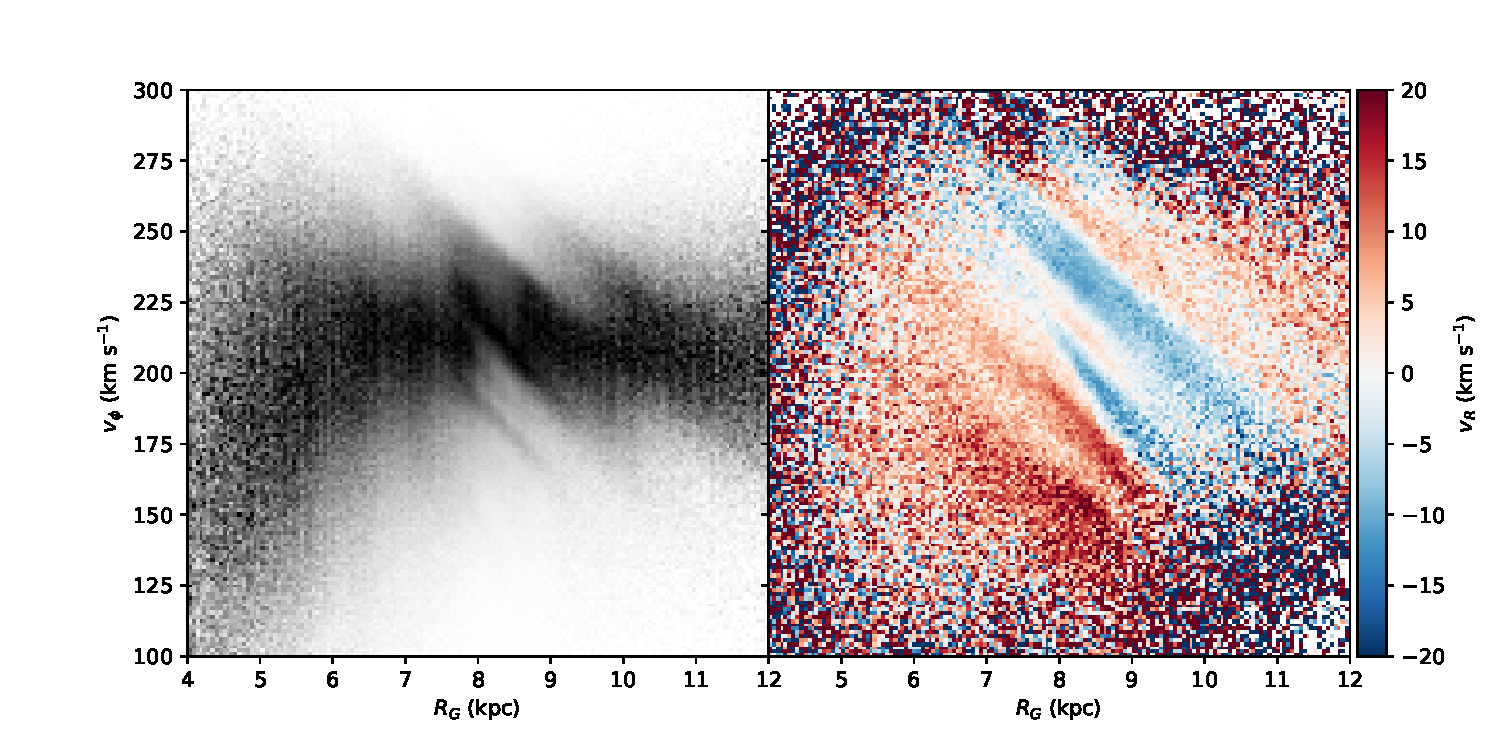
\includegraphics[width=\textwidth]{plots/gaia_RvT.pdf}
    \caption{$R$-$v_\phi$ plane in \textit{Gaia} DR2. \textbf{Left:} Number density of stars, normalized in each radial bin. \textbf{Right:} Mean Galactocentric radial velocities}
    \label{fig:gaia}
\end{figure}

For our test particle simulations, one of our main goals was to examine the conditions under which we can qualitatively reproduce these features in the Solar neighbourhood, and whether these features are due to resonances (e.g., due to the Galactic bar), or due to phase mixing induced by spiral arms. Here, we will provide a survey of a few of the models that we examined, and discuss how these qualitatively compare to the \textit{Gaia} data.

\subsection{Transient spiral arms with a long, slow bar}
One of the first models that we examined consisted of transient, winding spiral arms together with a long, slow Galactic bar. In particular, we examined a model with three cycles of $N=2$ winding spiral arms. The spiral arms were modelled with \texttt{galpy}'s \texttt{SpiralArmsPotential}, wrapped in a \texttt{CorotatingRotationWrapperPotential} as well as a \texttt{GaussianAmplitudeWrapperPotential} to simulate the winding and growth in amplitude. The Galactic bar was modelled with a \texttt{DehnenBarPotential}, and was given a radius of $R_b = 5$ kpc and a pattern speed of $\Omega_b = 1.3 \times \Omega_0$. Full details on the bar and spiral parameters can be found in \textcite{hunt2019}. For this model, the test particles were integrated for 10 bar periods, beginning from the formation time of the bar, and the growth of the bar lasted for 5 bar periods. For all of our models, we used \texttt{MWPotential2014} as the disk potential.

The time evolution of the $R$-$v_\phi$ plane, coloured by $v_R$, is shown in Figure \ref{fig:lsb}. The time steps range from $t = -417$ Myr to $t = 0$ Myr, where $t = 0$ is the present day. The integration was started at a negative time to maintain consistency with previous backward-time integration models with the same spiral and bar parameters. Each panel consists of a $30^\circ$ azimuthal wedge of test particles, centred on a constant $25^\circ$ offset from the Galactic bar. The spiral arms peak in amplitude at $t = -460$, $t = -230$, and $t = 0$ Myr.

\begin{figure}[h]
    \centering
    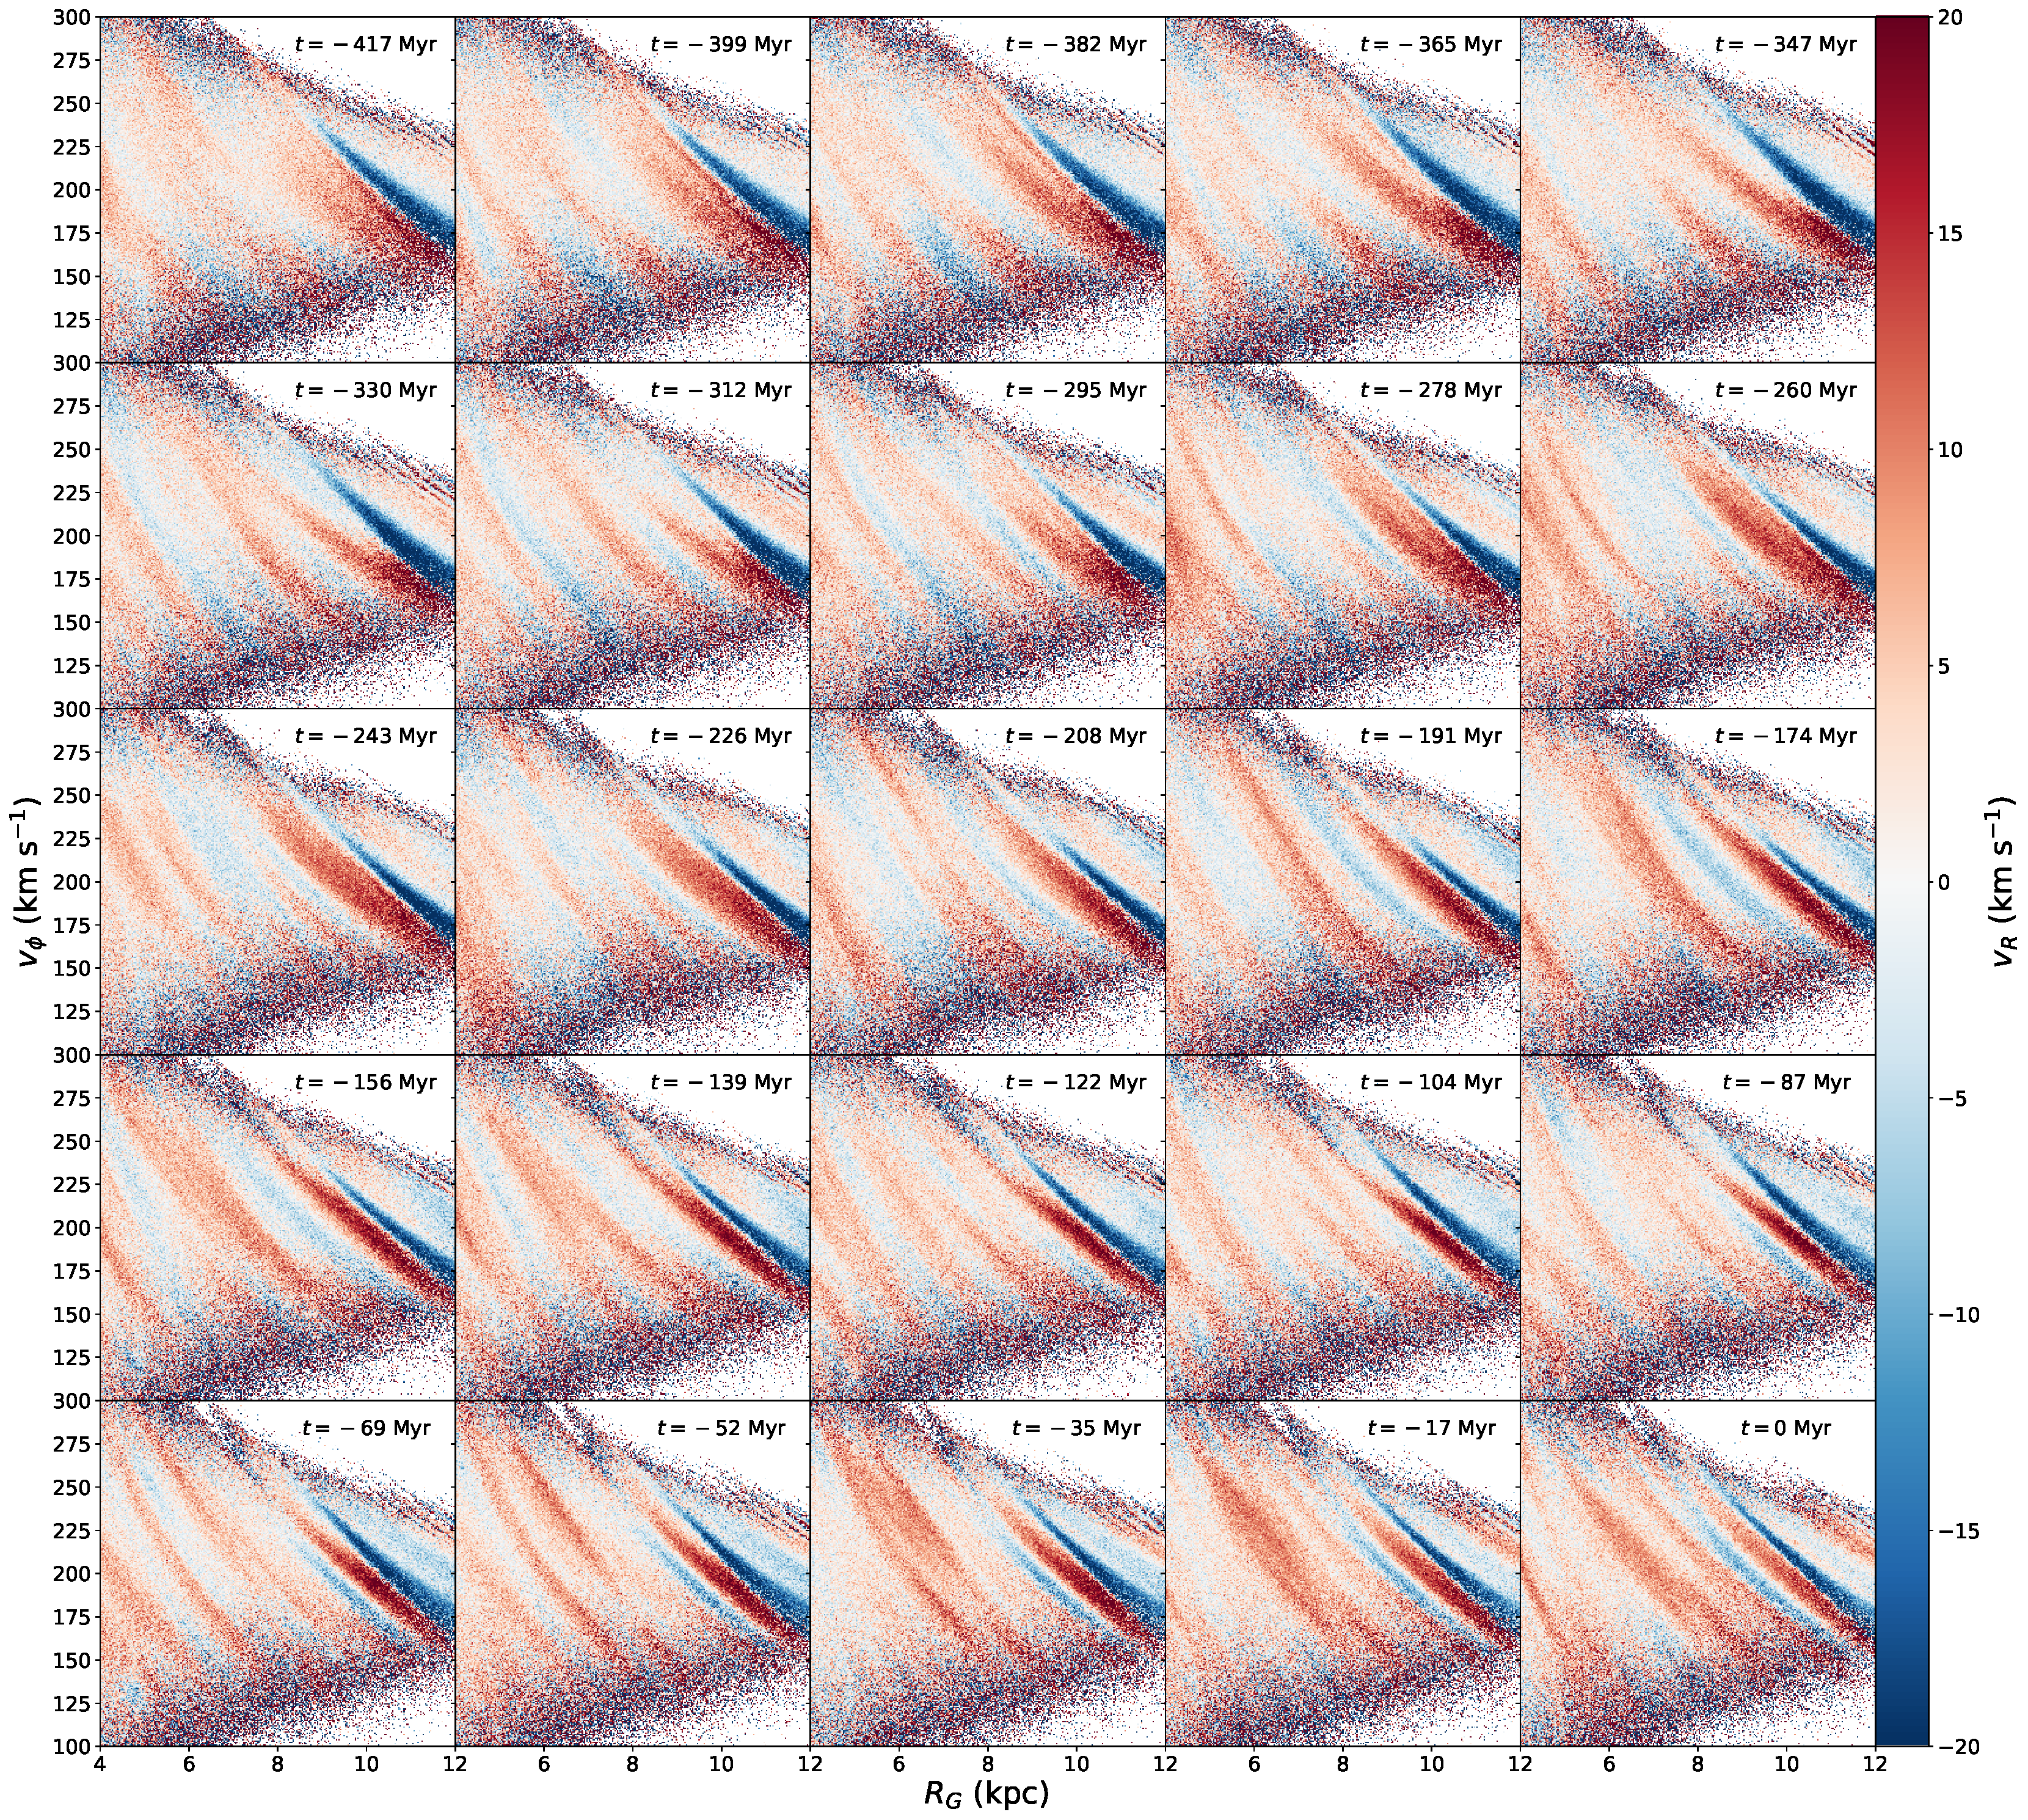
\includegraphics[width=\textwidth]{plots/base_spiral_RvT_vR.pdf}
    \caption{Time evolution of the $R$-$v_\phi$ plane, coloured by $v_R$, for the long, slow bar and transient spiral arms model.}
    \label{fig:lsb}
\end{figure}

In each panel, the outer Lindblad resonance (OLR) of the Galactic bar is the most prominent feature, appearing around $R_G = 10$ kpc with a strong inward-moving (blue) component toward larger $R_G$, as well as an outward-moving (red) component toward smaller $R_G$. It is never fully obscured by phase mixing due to the spiral arms, and the inward-moving component maintains its general tapering shape in each frame.

Toward the Solar neighbourhood, the model is not a particularly good fit to the \textit{Gaia} data. Although some panels can qualitatively reproduce one or two observed features (e.g., $t=-174$ contains a Sirius-like feature in approximately the right place, although it is thinner than in \textit{Gaia}), features in the model are consistently weaker than the observed data in the Solar neighbourhood. Moreover, few of the panels convincingly replicate the shape of the Hercules structure or the horn structure toward the Solar neighbourhood. The best reproduction of the tapering of the horn observed in \textit{Gaia} occurs at the OLR, however, its radial position is too large to be considered a good match to the data. For this reason, we decided to replace the long, slow bar with a short, fast bar, in the hopes that the OLR might better replicate the horn and Hercules features in the Solar neighbourhood.

\subsection{Transient spiral arms with a short, fast bar}
Our transient spiral arms for the short, fast bar were modelled similarly as for the long, slow bar model. However, the spacing between the spiral arms was adjusted slightly so that the spirals would originate from the bar, and also a larger pitch angle of $25^\circ$ was used, as compared to $12^\circ$ for the previous model. For the bar, we used a radius of $R_b = 3.3$ kpc and a pattern speed of $\Omega_b = 1.85 \times \Omega_0$. As before, we performed the integration for 10 bar periods from bar formation, and the growth of the bar lasted for 5 bar periods. 

The time evolution of the short, fast bar model is shown in Figure \ref{fig:sfb}. The time steps range from $t = -293$ Myr to $t = 0$ Myr, where the shorter time steps are owing to the faster pattern speed of the bar. As before, each panel is held at a constant $25^\circ$ offset from the bar. The spiral arms peak in amplitude at $t = -420$, $t = -210$, and $t = 0$ Myr.

\begin{figure}[h]
    \centering
    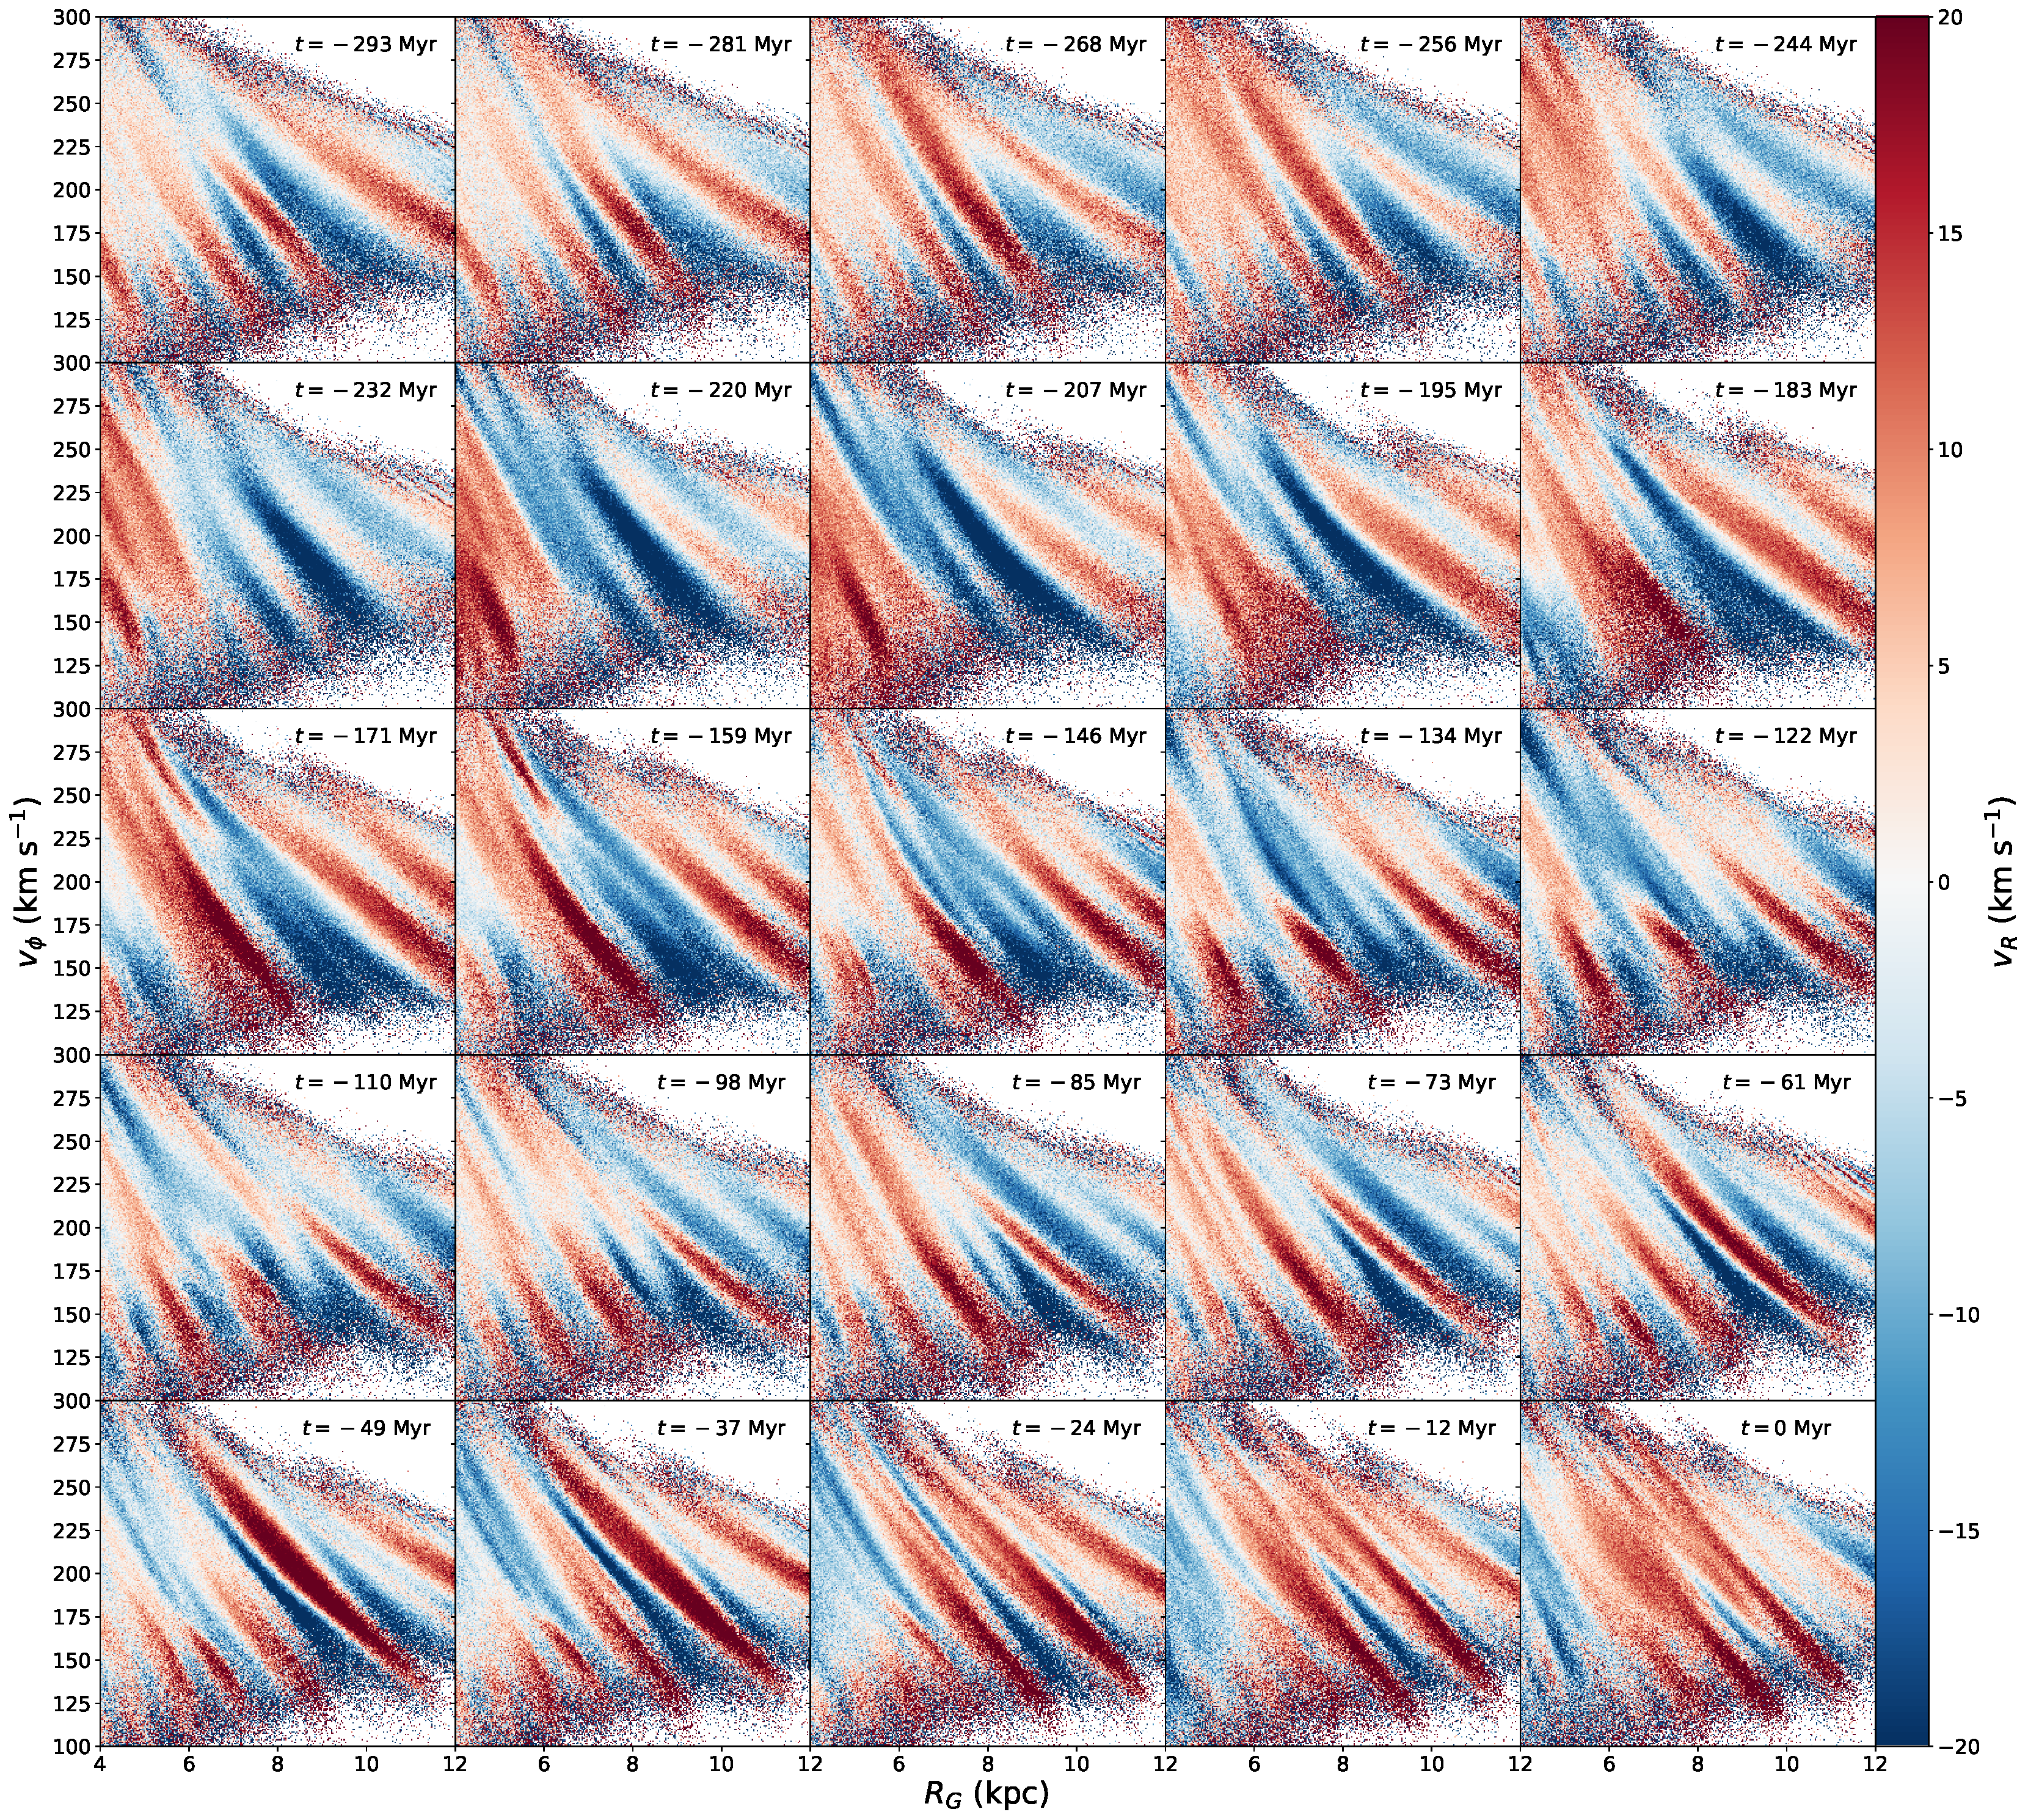
\includegraphics[width=\textwidth]{plots/sfb_spiral_RvT_vR.pdf}
    \caption{Time evolution of the $R$-$v_\phi$ plane, coloured by $v_R$, for the short, fast bar and transient spiral arms model.}
    \label{fig:sfb}
\end{figure}

In contrast to the previous model, the features in each frame are substantially stronger for this model. This is due to the different choice of pitch angle of the spiral arms, which has a strong effect on the strength of the phase mixing features. As a result, the OLR of the bar, which now appears closer to $R_G = 8$ kpc, is often significantly obscured by the phase mixing induced by the spiral arms, for instance at $t = -122$ Myr. Despite this, however, the inward-moving component of the OLR still maintains the tapering shape that was observed for the long, slow bar model, for instance at $t = -73$. 

The short, fast bar model has significantly better qualitative reproduction of the solar neighbourhood than the long, slow bar model. For instance, at $t = -73$ Myr, we see a good qualitative reproduction of the horn feature, a broad Sirius feature, an outward-moving Hercules, and Coma  Berenices. However, the features are all generally stronger than those observed in \textit{Gaia}, and Coma Berenices in particular appears much stronger than in the data. Also, Hercules appears substantially more elongated than in \textit{Gaia}, where it does not extend far above the ``height'' of the horn on the $v_\phi$ axis.

There is also good qualitative feature reproduction in some other time steps. For instance, $t = -159$ Myr reproduces a broad Sirius feature and a Hercules feature, although the tapering of the horn feature is not present, and a Coma Berenices feature is not visible. However, in general the phase mixing features are heavily time-dependent, and often do not last for more than three frames. Many frames, such as $t = 0$, are not a good fit to the Solar neighbourhood at all, and lack most of the key qualitative features. Given this, we also thought that it would be useful to examine the effect of the spiral arms alone, without the interference of a bar, to help decouple the effects of these two structures.

\subsection{Transient spiral arms with no bar}
To examine the effect of the spiral arms alone, we ran another model consisting of the spiral arms that were used in the long, slow bar model, but with the bar itself removed. The time evolution of this model is shown in Figure \ref{fig:no-bar}. The time steps range from $t = -178$ to $t = 0$ Myr. The time steps are fairly short because for this model, the integration began at $6 \sigma$ prior to the peak of the first spiral arm, where $\sigma$ is the lifetime of the spiral arms, which is a shorter overall integration time than the 10 bar periods of previous models. Nevertheless, the spiral arms follow the same parameters as used in Figure \ref{fig:lsb}, and peak at the same times. 

\begin{figure}[h]
    \centering
    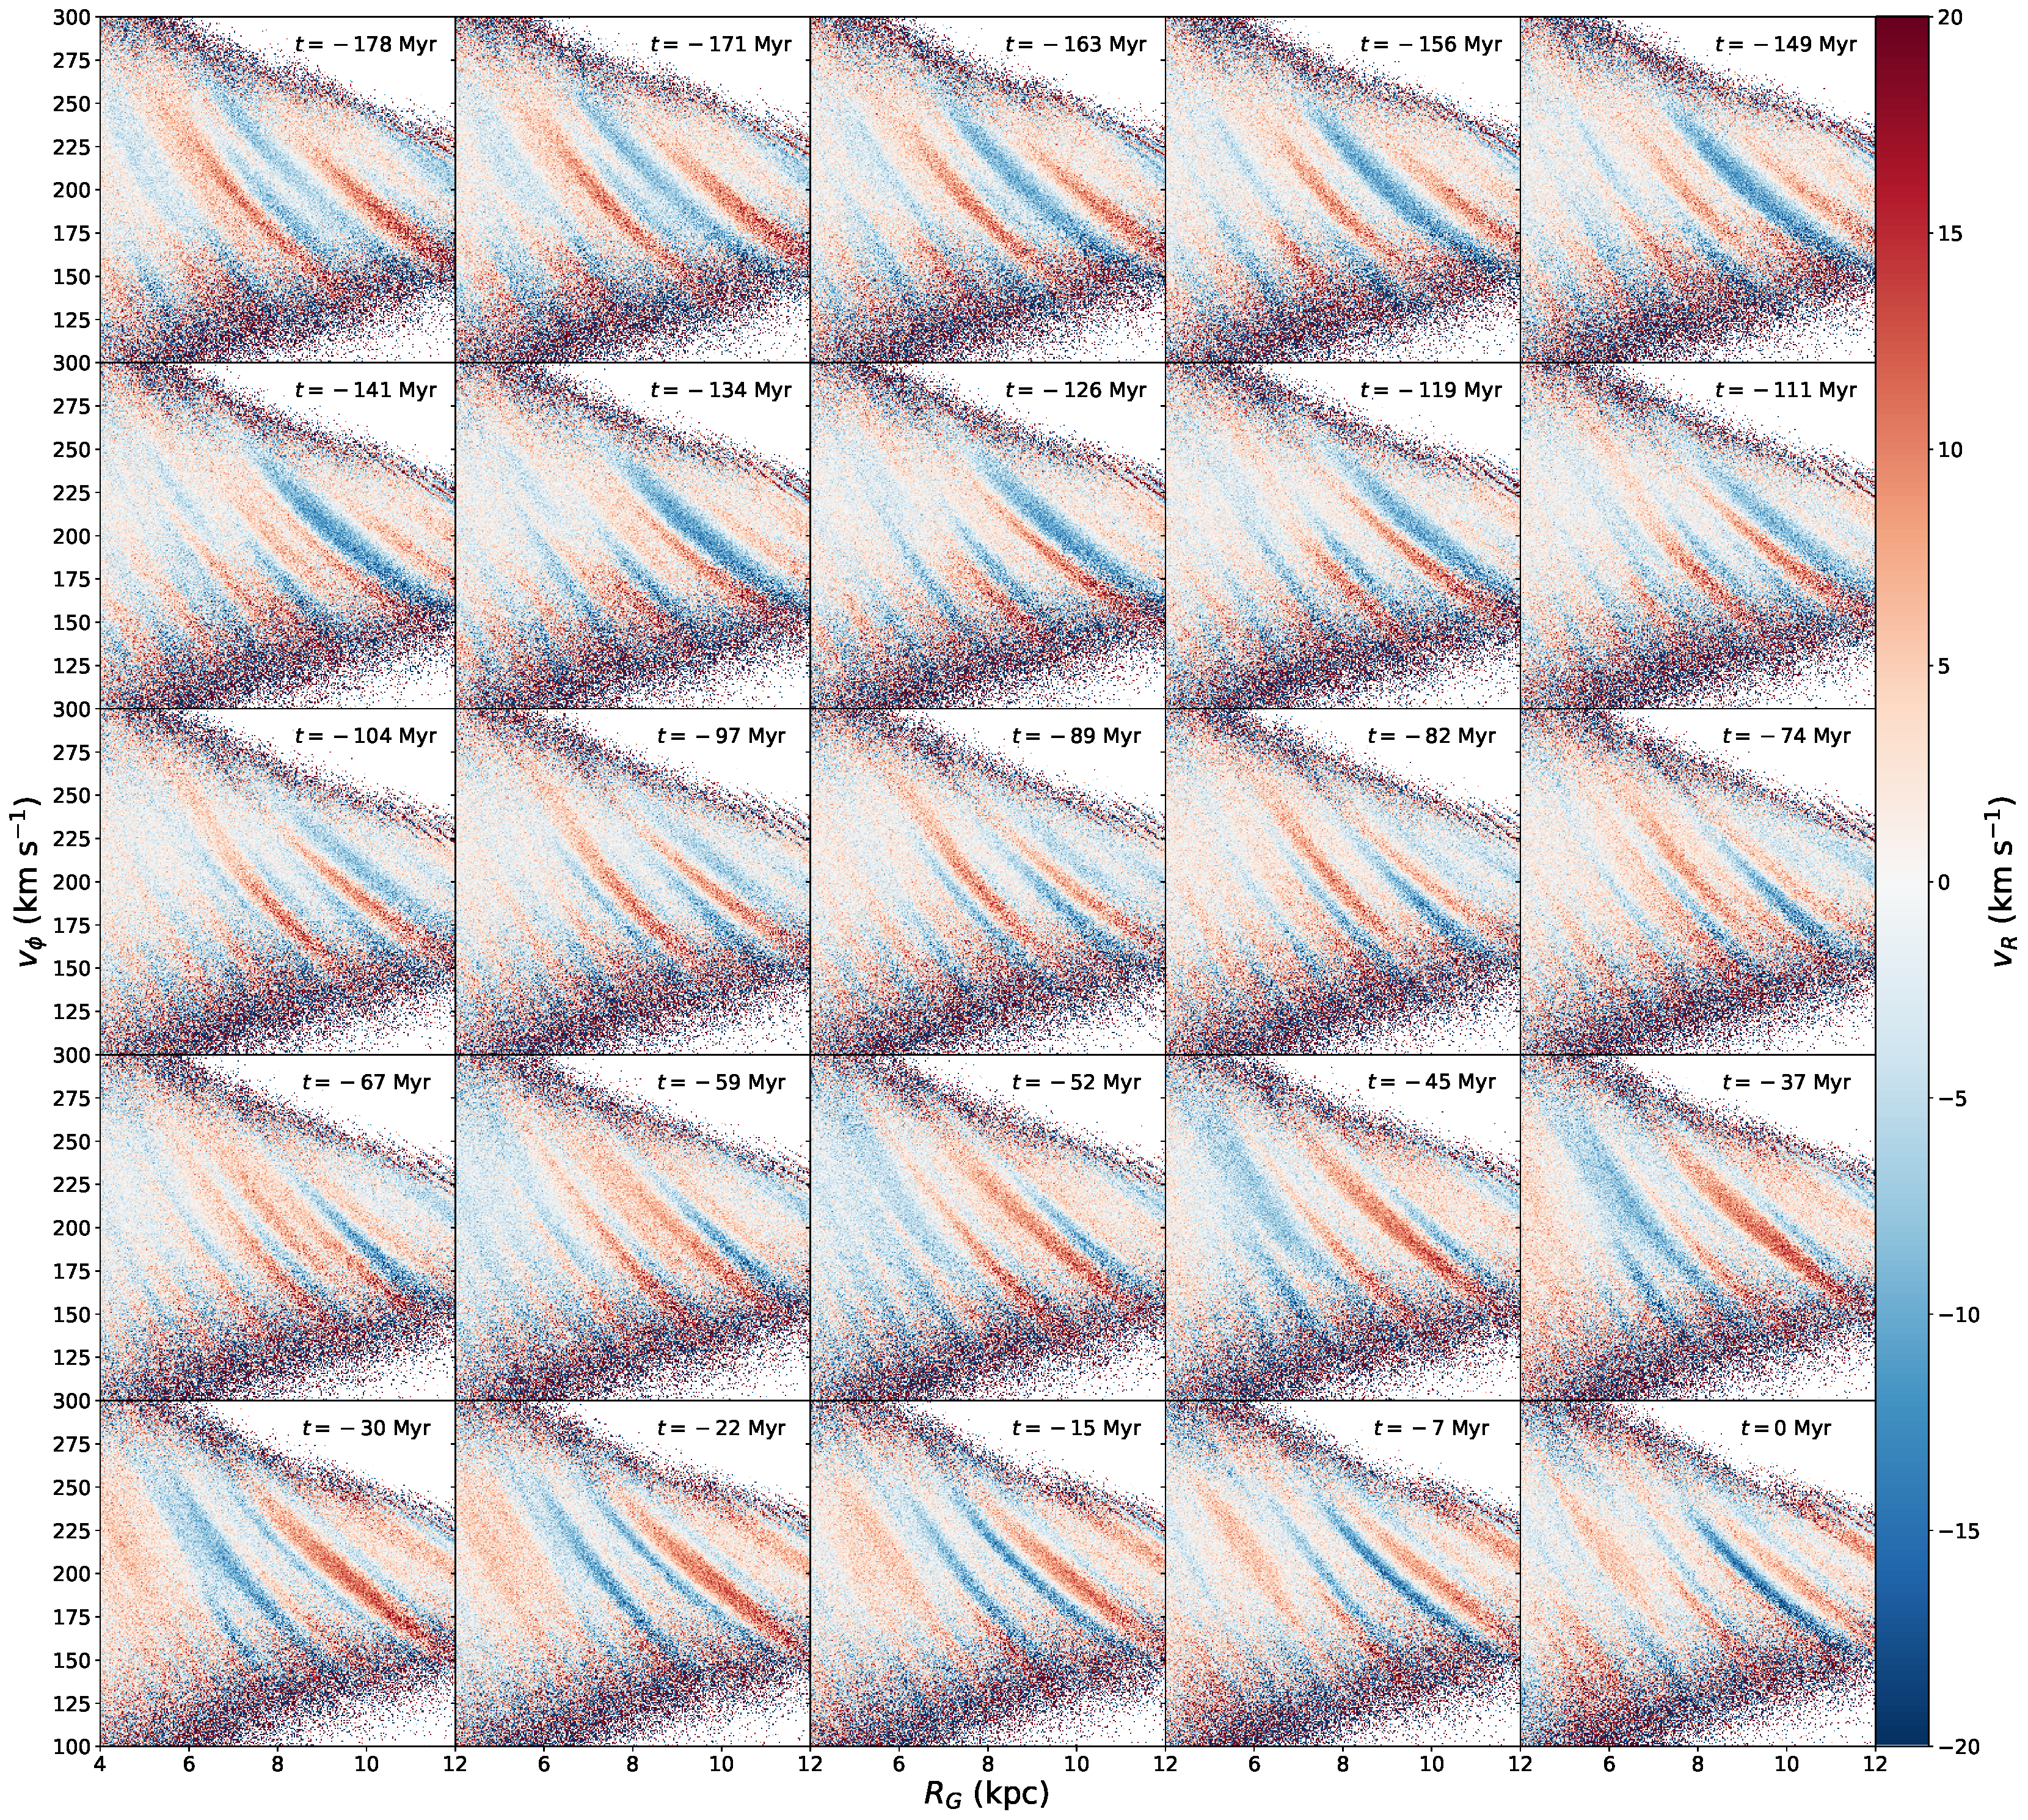
\includegraphics[width=\textwidth]{plots/three_spirals_no_bar_RvT_vR.pdf}
    \caption{Time evolution of the $R$-$v_\phi$ plane, coloured by $v_R$, for the transient spiral arms model with no bar. The spiral arm parameters are the same as those used in Figure \ref{fig:lsb}.}
    \label{fig:no-bar}
\end{figure}

Two notable features stand out in this model. First, we observe that the spiral arms alone are able to reproduce a broad, Sirius-like feature near $t = -134$ Myr in approximately the same location that it appears in $\textit{Gaia}$. This seems to support the possibility that this feature is a phase mixing effect due to the transient spiral arms. Second, we note that some frames, particularly $t = -178$ Myr, show a good reproduction of the Solar neighbourhood kinematics on their own. Here, we see a broad Sirius feature, an inward-moving feature in the same location as the horn, and an outward-moving feature in the same location as Hercules. This is somewhat concerning, as it becomes increasingly difficult to constrain the parameters of the bar and spiral arms given that many models can reproduce the Solar neighbourhood kinematics. However, as before, these features are all heavily time-dependent. In addition, none of the panels are able to make a convincing reproduction of the tapering shape of the horn structure visible in \textit{Gaia}. In our models, this tapering was always most convincingly reproduced by the OLR of the bar, which is obviously not present here.

We also examined the effect of individual spiral arms, prior to the beginning of the complex phase mixing induced by the multiple spiral cycles. Figure \ref{fig:single-spiral} shows an earlier time step of the no bar model, after the peak of the first spiral arm cycle, but prior to the peaks of the second and third cycles. Here, we can see that a single spiral arm cycle results in a regular alternation between outward- and inward-moving ridges in the $R$-$v_\phi$ plane, in contrast to the chaotic structures seen in prior figures. As such, it appears that the phase mixing features visible in Figure \ref{fig:no-bar} and others are due to the complex interactions of multiple spiral arm cycles, rather than a single spiral cycle alone. 

\begin{figure}[h]
    \centering
    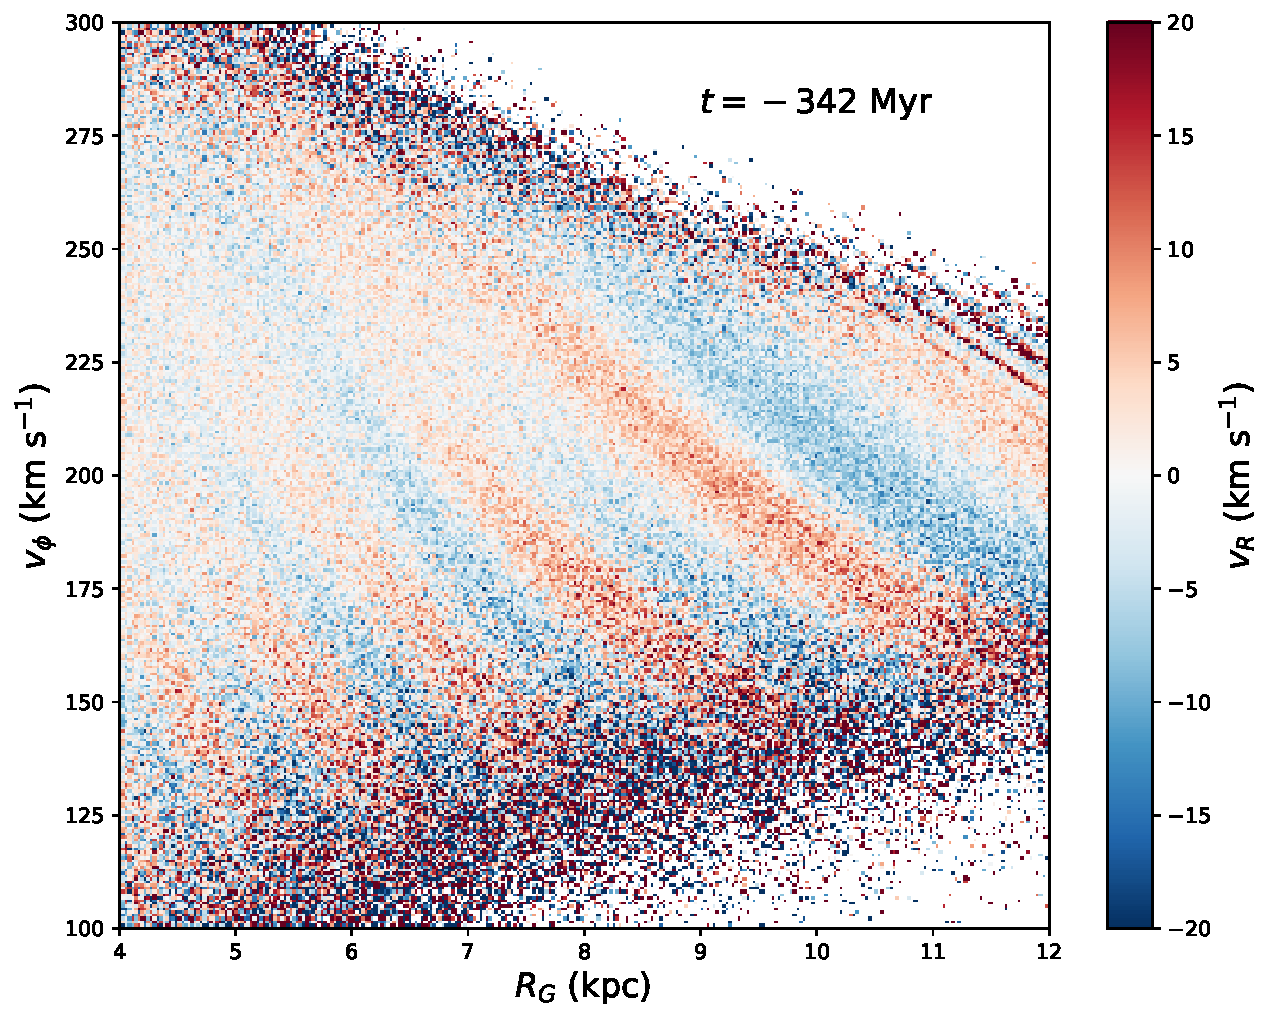
\includegraphics[width=\textwidth]{plots/single_spiral.pdf}
    \caption{An earlier time step of the model shown in Figure \ref{fig:no-bar}, after the peak of the first spiral, but shortly before the peaks of the second and third spirals.}
    \label{fig:single-spiral}
\end{figure}

\section{Conclusions}
The test particle simulations have provided several useful insights that are difficult to discover using the backward integration technique alone. In examining the $R$-$v_\phi$ plane for several transient spiral arm \& bar models, we have demonstrated that many of the structures seen in this plane are heavily time-dependent. Whereas in some time steps we find a good qualitative reproduction of the Solar neighbourhood kinematics, in others the reproduction is far less good. Further to this, we have also demonstrated that the chaotic nature of the phase mixing induced by the spiral arms allows several different types of models to reproduce the Solar neighbourhood kinematics, including a model consisting of solely transient spiral arms and nothing else. Although this is not good news for the purpose of constraining the bar and spiral arm parameters, it is useful to know the limits of our knowledge, and that we will likely need to rely on additional data before we can conclusively constrain the spiral arm parameters for the Milky Way.

Aside from the $R$-$v_\phi$ plane, the test particle simulations are generally useful for examining large-scale structure in the Galaxy and the time evolution of these structures. Therefore, there are many further applications of this technique that were not explored during the course of this project. As such, we anticipate that the techniques described herein will continue to be a helpful addition to future studies of the large-scale kinematic structure of the Galaxy.

\printbibliography
\end{document}